% put environments that should be ignored by texcount here, e.g., here lstlisting for code

%TC:envir lstlisting [] ignore

%for reference to this section
\section{Introduction}
\label{section:Introduction}

This paper aims to get a correlation between pedestrian traffic and route satisfaction. Given an open GPS Trajectories Dataset from the OpenStreetMap project, the research was conducted on the historical walking data in the City of Salzburg in Austria. Due to the city's historical growth, footpaths, pedestrian areas, and private and public transport roads are limited to change and urban development (SOURCE). 

\autocite[]{Netsch2021}

Historical traffic pattern mining and analysis for traffic forecasting and improving traffic flow is nothing new to vehicle traffic management. Multiple studies focus on collecting data, analyzing patterns, and forecasting traffic flow for vehicle traffic. 

Is it possible to increase satisfaction by recommending alternative, less populated routes to tourist attractions using pedestrian path model techniques?


\section{Background}
Lorem ipsum dolor sit amet, consectetur adipiscing elit. 

\section{Related Work}
Introduce why this specific related work is important for your own work. Which areas do you cover and why? What do you take as inspiration and what do you do differently/improve upon? 

\autocite[]{Sevtsuk2021}

\autocite[]{Delling2012}
\autocite[]{Hashemi2017}
\autocite[]{Qiu2015}
\autocite[]{Hendawi2019}
\autocite[]{Huber2016}

\section{Method}

A qualitative trail run will be conducted to measure a possible increase in satisfaction with the route proposal. In this trial run, a standard route will be compared to the newly proposed route and measured using two surveys. Survey number one uses a quantitative method to determine the subjects' general travel behavior, while survey number two compares and measures satisfaction with a quantitative approach after the trial run.

Finding out about the subjects' travel behavior should give a better understanding of the route proposal satisfaction survey results. Furthermore, it will give a relation to the subjects' travel behavior and the increase or decrease in satisfaction.

Qualitative Surveys.

Proposing the alternative route will be done by using the influence of historical pedestrian traffic to calculate a route with fewer interactions for the traveler to get to the same goal. This will be done by analyzing historical GPS trajectories and using a customized routing engine to propose the route for the trail run. through a GPS trace analysis and   


In present work, various research methods have been applied. They include a descriptive method (outlining different approaches to the term "actorness" and identifying the ways of measuring it), a historical method (following the historical development of the shared energy and environmental policies in the EU and their adaptation to the realities of the modern world), a comparative method (e.g., conferring the definitions of actorness and the level of actorness of the EU in energy and environmental spheres), statistical and quantitative (e.g., providing statistical data on the ecological goals and sustainable development, import of energy resources), analytical (e.g., assuming how the public opinion on the ecological situation contributes to the changing of the adopted energy policies), and process tracing method (e.g., identifying the causal mechanisms that link opportunity, presence, capability, performance, and effect, i.e., EU actorness).


Using the influence of traffic to propose an alternative route 

To be able to measure a possible increase in satisfaction of the route proposal a qualitative trail run of both routes will be conducted.

Therefore a route for the proposal to be compared to has to be found.

\section{System Overview}

Provide a high level overview of your system, approach, etc. 
Describe features, user interfaces, provide screenshots.
What does a user do with your application/system/interaction method?

Map Application

\section{Data Analysis}

To create the historical pedestrian traffic/walking patterns, a solid Data-set is needed so the routing engine can be configured to be adapted to the influence of the walking patterns. 

Searching for a Data-set that is viable for further analysis was not an easy task. There is no publicly available data from the city itself. Also, local research institutions contacted during the research period have no such data available. Therefore the OSM (OpenStreetMap) Project and its Database of public traces came in handy. Their collection is publicly accessible to be extracted, verified, classified, and then used to create a historical pedestrian traffic pattern for the part of the city that was used to create the alternative route.

% Struggles from Hashemi to relate here too.
% Cite:
%
%However, GPS traces are stored in plain text formats with no attached metadata such as, transpor- tation mode, length, or speed. This not only makes managing large volumes of GPS traces inefficient but also restricts the scale and scope of algorithms for human mobility pattern detection. Open Street Map (OSM), founded in UK in 2004 with more than 1 million registered users (Wood, 2013), is the most prominent volunteered geographic information devoted to providing a free map of the world empha- sizing the road networks. Road networks are built upon GPS traces uploaded by registered users and can be edited or updated manually at any time. A description can be associated to a GPS trace while being uploaded but there are no additional required metadata or restrictions (https://www.open- streetmap.org/traces; OpenStreetMap, n.d.). This means the transportation mode of the GPS trace (e.g. walking, motoring, or boating) cannot be known in the database which in turn limits the data- base’s applications. Besides, they do not store additional metadata, such as average speed or total length of the GPS trace which can be automatically calculated. Such metadata not only facilitates analyzing, mining, and visualizing large volumes of GPS traces, but also paves the path for automatic applications of GPS traces. Examples of such applications are automatic road and pedestrian network construction (Hashemi, 2017b), recognizing POIs (Bhattacharya, Kulik, & Bailey, 2015), developing intelligent location-based services (Liu & Karimi, 2006), detecting individual (Song et al., 2010), or collective (Becker et al., 2013; Harder, Nes, Jensen, Reinau, & Weber, 2012) mobility patterns, and real-time event detection which is of great value to municipalities, police, and fire departments.
%
%

The OSM Database of public traces consists of over 11 billion uploaded GPS points around the globe. \footnote{\url{https://planet.openstreetmap.org/statistics/data_stats.html}}

As the study's focus is the City of Salzburg, an appropriate bbox (Bounding box) covering the inner city and most of its close-to-be districts was selected. 

The reason for overlapping with towns and places around Salzburg is the OSM Editing API. Getting as many traces as possible leading into the city makes a more accurate estimation of pedestrian traffic possible. As the API is only taking routes that lead through the bbox , given a more extensive sample area than necessary for the route proposal was taken into account. The bbox taken is seen in Figure \ref{figure:BoundingBox}.

%figure* stretches figure over both columns
\begin{figure*}[t]
  \centering
  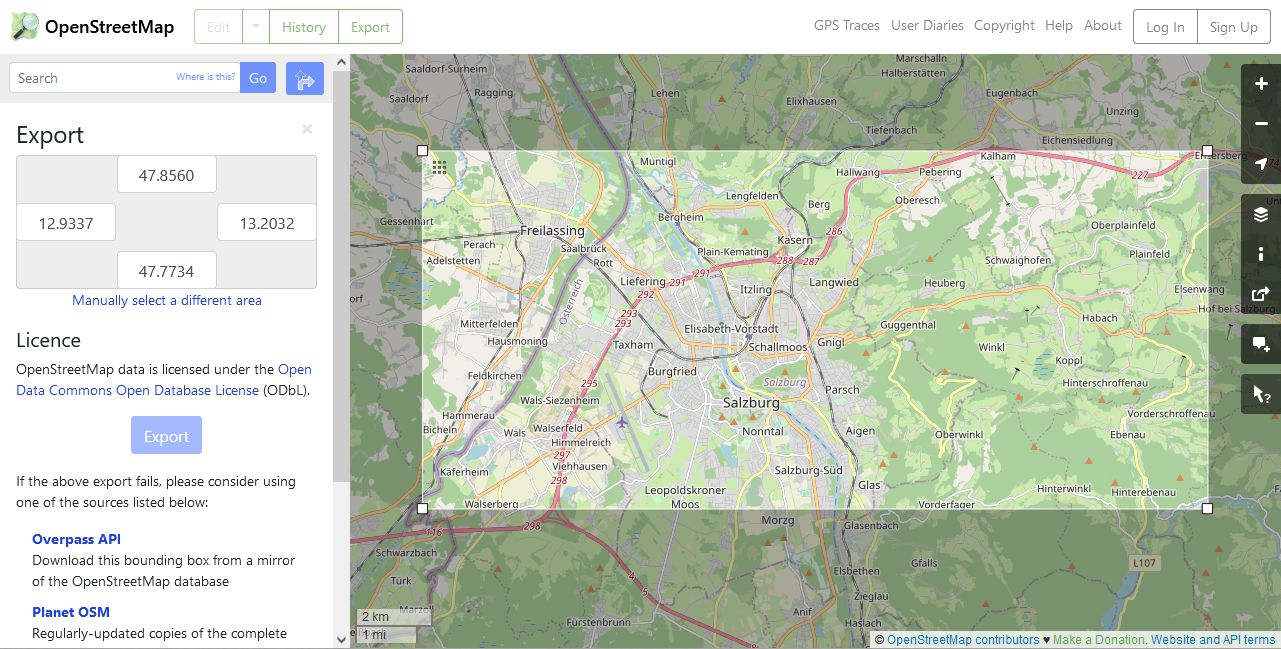
\includegraphics[width=0.9\textwidth]{images/BoundingBoxOSM.png}
  \caption{
  Bounding Box for extracted GPS trajectories.
  }
  %for reference to this figure
  \label{figure:BoundingBox}
\end{figure*}


\subsection{Data-set Overview}

Given the bbox of Salzburg and its surroundings, 1.173.334 Data-points were extracted using the OSM Editing API. \footnote{\url{https://wiki.openstreetmap.org/wiki/API_v0.6#GPS_traces}}

The OSM Editing API is a collection of APIs based on RESTful API principles. There are API calls to create, read, update, and delete the three fundamental elements that makeup OpenStreetMap's map data. They each return or expect the data for the elements in an XML format.
\autocite[]{wiki:xxx}

The Data-points are returned using GPX (GPS Exchange Format) a XML data format for GPS data \footnote{\url{https://www.topografix.com/GPX/1/1/#type_trksegType}}. Important to mention is that in violation of the GPX standard, for privacy reasons, all waypoints of non-trackable traces are randomized and delivered as one track segment. 

GPX (the GPS Exchange Format) is a light-weight XML data format for the interchange of GPS data (waypoints, routes, and tracks) between applications and Web services on the Internet. 

Important to mention is that This happens in violation of the GPX standard. 

To further work with the data points 

\subsection{Data Extraction}

\begin{lstlisting}
<?xml version="1.0" encoding="UTF-8"?>
<gpx version="1.0" creator="OpenStreetMap.org" xmlns="http://www.topografix.com/GPX/1/0">
    <trk>
        <name>osmtrack_KUnrl0ZaKm.gpx</name>
        <desc>desc.</desc>
        <url>/user/exbrick/traces/3444105</url>
        <trkseg>
            <trkpt lat="47.8318200" lon="13.0567170">
                <time>2006-08-22T01:37:05Z</time>
            </trkpt>
            <trkpt lat="47.8325810" lon="13.0567800">
                <time>2006-08-22T01:37:20Z</time>
            </trkpt>
            <trkpt lat="47.8331180" lon="13.0569120">
                <time>2006-08-22T01:37:30Z</time>
            </trkpt>
            
\end{lstlisting}

\section{Model & Implementation}

Provide implementation details such as the used software and our software architecture, highlight your own solutions to encountered difficulties. Describe relevant iterations of your implementation.

Before going deeper into the system architecture 
To go deeper into the system architecture 
Overview of the software basis used for the whole development: 
NodeJS, React,

Providing a route proposal starts further than analyzing geo-located trajectories. Precautious steps were needed in building the architecture to understand the data used for the newly suggested route. 

Therefore a Map Application was created to visualize the extracted and classified data, the routes used for the comparison, and the new suggested routes from the utilized routing engine. Said Map Application is a standalone React App using the Mapbox Plattform for map creation and route visualization. For working with React, Mapbox provides mapbox-gl-js, a javascript library that uses WebGL to render interactive maps from vector tiles and Mapbox styles.

%https://www.mapbox.com/
%https://docs.mapbox.com/mapbox-gl-js/guides/

For the map and route visualization to interact with the extracted geo trajectory data, a NodeJS backend was developed. The backend interacts with the OSM API and the established GeoDatabase, handling the trajectories' extraction, classification, and transformation.

With its geospatial data support, MongoDB was selected as the Geo-Database and stores the extracted Data-Set and the further classified data objects. Even though PostGIS is more mature and built on the Open Geospatial Consortium (OGC) standards, the uncertainty of incomplete data sets from the OSM project led to the decision to use the document-based solution.

To work with the OSM project and its map data, the JOSM (Java OpenStreetMap editor) was used to interact with the map layer as the basis for the route proposal. 
%https://josm.openstreetmap.de/

For the data extraction, a NodeJS backend interacting with the OSM API and the established GeoDatabase was created, handling the extraction, classification, and visualization of the trajectories and route suggestions.

Therefore a visualization of the City of Salzburg was built using the Mapbox Plattform. 
% https://docs.mapbox.com/mapbox-gl-js/guides/



% https://wiki.openstreetmap.org/wiki/Bounding_Box

\subsection{Database}

After the conversion the objects 
Working with Geodata there is 

MongoDB & Mongoose
% https://mongoosejs.com/docs/geojson.html
% https://www.mongodb.com/docs/manual/reference/geojson/

\subsection{Data Extraction}

Working with the OSM API

To retrieve the GPS track points 

https://api.openstreetmap.org/api/0.6/trackpoints?bbox=12.9337,47.7564,13.2032,47.8560&page=0

Get GPS Points: Get /api/0.6/trackpoints?bbox=left,bottom,right,top&page=pageNumber
Use this to retrieve the GPS track points that are inside a given bounding box (formatted in a GPX format).

Get GPS Points: Get /api/0.6/trackpoints?bbox=left,bottom,right,top&page=pageNumber


Use this to retrieve the GPS track points that are inside a given bounding box (formatted in a GPX format).

where:

left, bottom, right, and top are used the same way as they are in the command to retrieve nodes, ways, and relations.

pageNumber specifies which group of 5,000 points, or page, to return. Since the command does not return more than 5,000 points at a time, this parameter must be incremented—and the command sent again (using the same bounding box)—in order to retrieve all of the points for a bounding box that contains more than 5,000 points. When this parameter is 0 (zero), the command returns the first 5,000 points; when it is 1, the command returns points 5,001–10,000, etc.

% https://www.topografix.com/GPX/1/1/#type_trksegType

\subsection{Data Prepocessing}

Conversion

As the objects returned from the API are in the GPX Format, a conversion step was needed to further work with the trajectories. As the MongoDB Database and the libraries used in the built Map Application are working with the GeoJSON standard \footnote{\url{https://datatracker.ietf.org/doc/html/rfc7946}}, a conversion step was necessary.

The conversion was achieved using the toGeoJSON tool \footnote{\url{https://github.com/mapbox/togeojson}} provided by Mapbox. After the first objects were converted, a significant number of them had attributes missing after the conversion.  Therefore, the tool was adapted according to the GPX Formats' given attributes used by the OSM API.  

Attributes added: Properties

Using the tool togeojson provided by Mapbox the conversion was 

% https://github.com/mapbox/togeojson

\subsection{Map-Matching}



\subsection{Data Classification}


TurfJS





osrm

Mapbox API



\subsection{Reverse Geo-coding}

nominatim

\subsection{Routing}

Routing Engine

\autocite[]{Delling2012}


\section{}

\section{Evaluation}
Describe your methodology. How did you evaluate your work? Why did you choose this methodology? Present results of your evaluation here.

\section{Discussion}
Discuss your results to answer your research question. Does your data support you hypotheses? Put your results into perspective by situating it in the research field/related work.

\section{Conclusion and Future Work}
Summarize your work, outline limitations and future work. 

% \section{Formatierung}
% \label{section:Formatting}

% Text mit beliebigen Sonderzeichen in UTF-8 ohne BOM \ldots
% ,
% \textbf{hervorgehobener Text},
% \texttt{void}\footnote{Fußnote 1},
% mathematische Formel im Text $\sum_{i=0}^n i^2$
% \ldots

% Referenz auf Unterabschnitt \ref{subsection:Coding} der Arbeit, automatisch richtig nummeriert.

% \textcite[]{Mulloni:2010} für einen einen Literaturverweis im laufenden Text.

% Literaturverweise sind essentiell für eine wissenschafliche Arbeit. \autocite[]{McConnell:2004:CCS:1096143}.

% Achtung: nur zitierte Literatur wird im Literaturverzeichnis
% angeführt.\footnote{Fußnote 2}


% Wir verwenden \LaTeX\footnote{ \url{http://en.wikibooks.org/wiki/LaTeX}} -- und das
% ist keine Quelle, sondern blos eine URL.

% \subsection{Figures machen was sie wollen}

% % h = try to place the figure Here
% % t = try to place the figure at the Top of a page
% % p = try to place this figure along with others on a separate Page
% % Note that LaTeX has a sophisticated ranking algorithm to place figures.
% % It is not always easy to accept LaTeX's placing but it is harder doing it
% % manually. Just let it go ;-)
% \begin{figure}[!ht]
% 	\centering
% 	\subfloat[Das Julia Fraktal]{
% 		\includegraphics[width=0.75\linewidth]{images/Julia-Fractal.png}
% 		%for reference of this subfigure only
% 		\label{subfigure:Julia-Fractal}
% 	}
% 	\qquad
% 	\subfloat[Noise für Tinteneffekte]{
% 		\includegraphics[width=0.75\linewidth]{images/Perlin-Coherent.png}
% 		%for reference of this subfigure only
% 		\label{subfigure:Perlin-Coherent}
% 	}
% 	\caption[
% 		Verschiedene Pixelgraphiken\newline
% 		% source url given in the table of figures
% 		\small\texttt{https://mediacube.at/wiki/}
% 	]{
% 		Verschiedene Pixelgraphiken
% 	}
% 	%for reference to all subfigures
% 	\label{figure:PixelImages}
% \end{figure}

% Unterstützte Pixelgraphikformate: PNG, JPEG, PDF.
% Angabe von height oder width meist wichtig.

% Referenz auf Abbildung \ref{figure:PixelImages} mit allen Teilbildern.
% Referenz auf Unterabbildung \ref{subfigure:Julia-Fractal}.

% %figure* stretches figure over both columns
% \begin{figure*}[t]
% 	\centering
% 	\includegraphics[width=0.9\textwidth]{images/KappaGamma.pdf}
% 	\caption{
% 		Vektorgraphik mit \LaTeX\ Beschriftung ($\kappa$, $\gamma$)
% 	}
% 	%for reference to this figure
% 	\label{figure:KappaGammaTau}
% \end{figure*}

% Referenz auf Abbildung \ref{figure:KappaGammaTau}.

% Bei Vektorgraphik mit \LaTeX\ Beschriftung keine Skalierung mit width oder height verwenden.

% Vektorgraphik mit \LaTeX\ Beschriftung kann etwa mit \texttt{ipe} erstellt werden.

% Unterstütztes Vektorgraphikformat: PDF. EPS muss konvertiert werden.


% \subsection{Unterabschnitt 2}
% %for references to this subsection
% \label{subsection:Coding}

% \begin{lstlisting}[
% 	label=listing:Main, %for reference to this listing
% 	float=h,
% 	caption=main.cpp,
% 	firstnumber=10
% ]
% int main(void) {
% 	while (true) {
% 	}
% 	return 0;
% }
% \end{lstlisting}

% Wie man in Listing \ref{listing:Main} in Zeile 10 sieht, kann man die Zeilennummern im Listing absichtlich setzen, hier z.B. auf 10. In Listing \ref{listing:closure} wurde davon nicht Gebrauch gemacht. In diesem Fall beginnt die Nummerierung bei 1.

% \begin{lstlisting}[
%     label=listing:closure,
% 	float=h,
% 	caption=Closure in Javascript,
% 	language=JavaScript
% ]
% function foo(x,y) {
%     let i = x;
%     return function(a) {
%         return i * 2;
%     }
% }
% \end{lstlisting}


% \subsubsection{Unterunterabschnitt i}

% Wörtliches Zitat:
% %select proper language if not in German
% \selectlanguage{english}
% \begin{quote}
% ``Erwin Unruh discovered that templates can be used to compute
% something at compile time. [...] The intriguing part of this exercise, however, was that the production of the prime numbers was performed by the compiler during the compilation process and not at run time.''

% \autocite[305]{Bosch2014}
% \end{quote}
% %select German again or the language that you were using before (note ngerman stands for New German)
% %\selectlanguage{ngerman}
% \selectthesislanguage


% \subsection{Unterabschnitt b}

% \begin{enumerate}
% 	\item Punkt 1
% 	\begin{enumerate}
% 		\item Unterpunkt 1
% 		\item Unterpunkt 2
% 	\end{enumerate}
% 	\item Punkt 2
% \end{enumerate}

% \begin{itemize}
% 	\item Punkt 1
% 	\begin{itemize}
% 		\item Unterpunkt 1
% 		\item Unterpunkt 2
% 	\end{itemize}
% 	\item Punkt 2
% \end{itemize}


% \subsection{Unterabschnitt c}

% \begin{table}[ht]
% 	\centering
% 	\begin{tabular}{r|rrr}
% 		    & $i$ & $j$ & $k$ \\ \hline
% 		$i$ &$-1$ & $k$ &$-j$ \\
% 		$j$ &$-k$ &$-1$ & $i$ \\
% 		$k$ & $j$ &$-i$ &$-1$
% 	\end{tabular}
% 	\caption{
% 		Multiplikationstabelle für Quaternionen
% 	}
% 	\label{table:Quaternions}
% \end{table}

% Referenz auf Tabelle \ref{table:Quaternions}.

% \section{Abschnitt 2}
% \label{section:MathematicalStuff}

% Sei $f(x)$ eine stetige Funktion, so ist die \textbf{Fourier Transformierte}
% $F(\omega)$ wie folgt definiert:
% \begin{equation}
% \label{equation:FourierDefinition}
% 	F(\omega) = \int_{-\infty}^{\infty} f(x) e^{-i\omega t} dt
% \end{equation}

% Referenz auf mathematische Gleichung (\ref{equation:FourierDefinition}).

% Unnummerierte Gleichung:
% \begin{equation*}
% 	e^{i\varphi} = \cos\varphi + i \sin\varphi
% \end{equation*}
% %you may also use \[ \] instead of \begin{equation*} and \end{equation*}

% Gleichungssystem:
% \begin{eqnarray}
% 	g(x) = f(x - x_0) & \Leftrightarrow &
% 		G(\omega) = F(\omega) e^{-i\omega x_0} \\
% 	g(x) = f(x) e^{i\omega_0 x} & \Leftrightarrow &
% 		G(\omega) = F(\omega - \omega_0)
% \end{eqnarray}
